%!TEX root = start.TEX
\section{Marco teórico}
\subsection{Aprendizaje Profundo}
\frame{

	\begin{block}
	{\Large{Aprendizaje Profundo}}
	\end{block}
	\vskip 0.5cm
	\begin{itemize}
	\item<1-> {\bf Aprendizaje Profundo}
	\begin{itemize}
	\item<2->  El verdadero desafío para la inteligencia artificial fue y es resolver las tareas que son fáciles de realizar para las personas pero difíciles de describir de manera formal, problemas que resolvemos intuitivamente, que se sienten automáticos, como reconocer palabras, rostros u objetos en las imágenes \citep{Goodfellow-et-al-2016}.
	\vskip 0.3cm
	\item<3->El aprendizaje automático es considerada como la mejor técnica de la inteligencia artificial(IA); es decir, es el campo de la IA que hoy en día muestra la mayor promesa al proporcionar herramientas que la industria y la sociedad pueden usar para producir algún cambio. 

	\vskip 0.3cm
	\item<4-> En tal sentido,el aprendizaje automático toma algunas de las ideas centrales de la inteligencia artificial y las enfoca en resolver problemas del mundo real con redes neuronales diseñadas para imitar nuestra propia toma de decisiones. 
	\end{itemize}
	\end{itemize}
}

\frame{
\begin{block}
{\Large{Aprendizaje Profundo}}
\end{block}
	
	\begin{itemize}
	\item<1->Por otro lado, el aprendizaje profundo o avanzado de máquinas (del inglés, {\bf deep learning}) se centra aún más estrechamente en un subconjunto de herramientas y técnicas del aprendizaje automático y los aplica a la solución de casi cualquier problema que requiera "pensamiento", ya sea humano o artificial.
	\vskip 0.2cm
	\item<2->Se puede sostener que el aprendizaje automático es el único enfoque viable para construir sistemas de inteligencia artificial que puedan operar en entornos complicados del mundo real y el {\bf aprendizaje profundo} es, a su vez, un tipo particular de aprendizaje automático que logra gran poder y flexibilidad al representar el mundo como una jerarquía de conceptos anidados, con cada concepto definido en relación con conceptos más simples y representaciones más abstractas calculadas en base a representaciones menos abstractas.
	% La siguiente es un diagrama de Venn que muestra cómo el aprendizaje profundo es una especie de aprendizaje de representación, que a su vez es una especie de aprendizaje automático, que se utiliza para muchos, pero no todos los enfoques de la IA. 
	\end{itemize}
}

\frame{
\begin{block}
{\Large{Aprendizaje Profundo}}
\end{block}
\begin{figure}[H]
		\begin{center}
		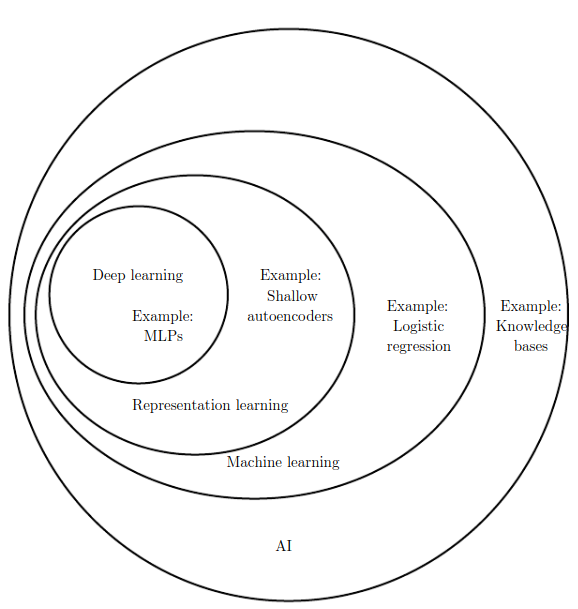
\includegraphics[width=0.7\textwidth,height=0.65\textheight,keepaspectratio]{images/marcoteorico/venn_diag}
		\vskip -2cm
		\end{center}
		\begin{center}
		\caption{\small{Diagrama de Venn donde cada sección incluye un ejemplo de una tecnología de IA(ilustra la relación entre estas diferentes disciplinas de la IA)}}
		\vskip -0.2cm
		{\small{Fuente: \citep{Goodfellow-et-al-2016}}}
		\end{center}

	\end{figure}
}

%	Para muchas tareas, sin embargo, es difícil saber qué características se deben extraer. Por ejemplo, un programa para detectar automóviles en fotografías. Se sabe que los autos tienen ruedas, por lo que sería importante utilizar la presencia de una rueda como característica. Desafortunadamente, es difícil describir exactamente cómo es una rueda en términos de valores de píxel. Una rueda tiene una geometría simple, pero su imagen puede verse complicada por las sombras que caen sobre la rueda, el sonido de las partes metálicas de la rueda, el guardabarros del automóvil o un objeto en el primer plano que oscurece la rueda, y así sucesivamente. 



\frame{
\begin{block}
{\Large{Aprendizaje Profundo}}
\end{block}
	
	\begin{itemize}
	\item<1->El aprendizaje profundo es un enfoque específico utilizado para construir y entrenar redes neuronales para la toma de decisiones altamente prometedoras, \citep{Goodfellow-et-al-2016}.

	\item<2->Se considera que un algoritmo es profundo si los datos de entrada se pasan a través de una serie de no linealidades o transformaciones no lineales antes de que se emita. 

	\item<3->Este enfoque permitir que las computadoras aprendan de la experiencia y entiendan el mundo en términos de una jerarquía de conceptos, con cada concepto definido a través de su relación con conceptos más simples. 

	\item<4->Al reunir el conocimiento de la experiencia, este enfoque evita la necesidad de que los operadores humanos especifiquen formalmente todo el conocimiento que necesita la computadora.
	\end{itemize}
}


\frame{
\begin{block}
{\Large{Aprendizaje Profundo}}
\end{block}
	\begin{figure}[H]
		\begin{center}
		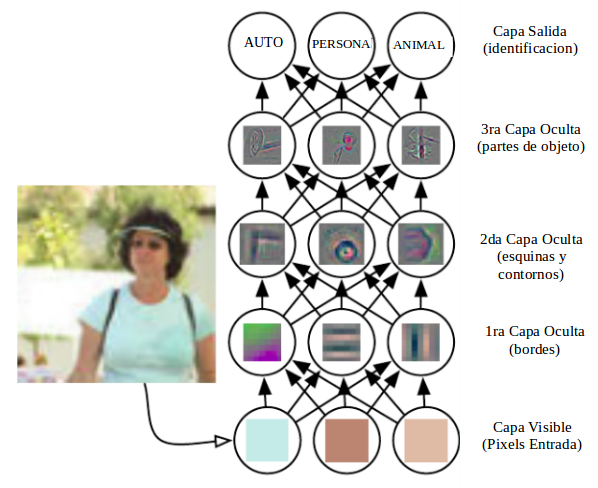
\includegraphics[width=0.7\textwidth,height=0.65\textheight,keepaspectratio]{images/marcoteorico/deepExam}
		\end{center}
		\vskip -0.5cm
		\begin{center}
		\caption{\small{El aprendizaje profundo permite a la computadora construir conceptos complejos a partir de conceptos más simples}}
		\vskip -0.2cm
		{\small{Fuente propia}}
		\end{center}
	\end{figure}
}


%-----------------%-----------------Red Convolucional-----------------%-----------------
\subsection{Red Convolucional}
\frame{
\begin{block}
{\Large{Red Convolucional}}
\end{block}

		\begin{itemize}
			\item<1->Nueve de cada diez veces, cuando se escucha que el aprendizaje profundo rompe una nueva barrera tecnológica, las redes neuronales convolucionales están involucradas. También llamados CNN(del inglés , {\bf Convolutional Neural Networks}) o  {\bf ConvNets}, estas son las preferidas del campo de redes neuronales profundas. Han aprendido a clasificar las imágenes en categorías incluso mejor que los humanos en algunos casos, \citep{Rohrer}.
			\vskip 0.5cm
			\item<2-> Estas son muy similares a las redes neuronales ordinarias, están formadas por neuronas que tienen pesos y biases(sesgos) que se pueden aprender durante el entrenamiento de estas. Cada neurona recibe algunas entradas y realiza operaciones matemáticas.
		\end{itemize}
}


\frame{
\begin{block}
{\Large{Red Convolucional}}
\end{block}
		\begin{itemize}
			\item<1->Una ConvNet se caracteriza por tener una secuencia de capas donde cada una de estas transforma un volumen de activaciones en otro nuevo a través de funciones y el aprendizaje profundo se produce cuando se utilizan varias de estas capas variando los parámetros de configuación dentro y entre dichas capas. 
			\vskip 0.5cm
			\item<2->El resultado de las CNNs es que pueden encontrar si una característica está en una imagen sin preocuparse exactamente de donde está. Esto ayuda a resolver el problema de las computadoras al comparar imágenes de manera hiper-literal, es decir, que coincida pixel a pixel para que se trate de imágenes iguales.
			%\vskip 0.5cm
		\end{itemize}
}




\frame{
\begin{block}
{\Large{Red Convolucional}}
\end{block}
		\begin{figure}[H]
		\begin{center}
		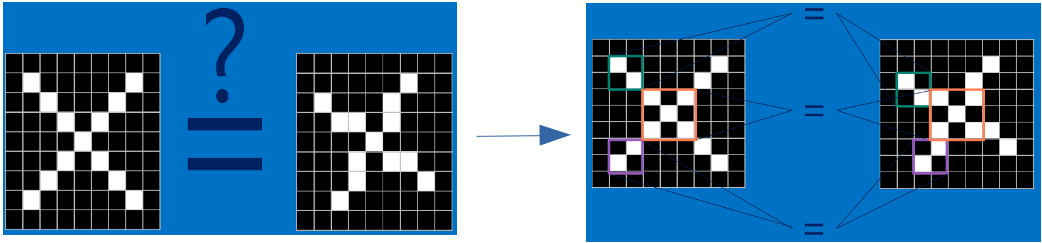
\includegraphics[width=0.8\textwidth]{images/marcoteorico/literalcomp}
		\end{center}
		\begin{center}
		\caption{\small{Analisis de una CNN}}
		\vskip -0.25cm
		{\small{Fuente: \citep{Rohrer}}}
		\end{center}
		\vspace{-1.5em}
		\end{figure}

}

%--------------------Red Convolucional - Terminologías-------------------------
\frame{
\begin{block}
{\Large{Red Convolucional}}
\end{block}
	\begin{itemize}
	\item<1-> {\bf Red Convolucional - Terminologías}
			\vskip 0.5cm
		\begin{itemize}
			\item<2->Una es cuando la red convolucional es vista como un número largo de capas simples y cada paso del procesamiento se considera como una capa en sí misma. 
			\vskip 0.5cm
			\item<3->Otra terminología es cuando la red convolucional es vista como un número pequeño de capas relativamente complejas, donde cada capa tiene multiples etapas.
			
		\end{itemize}
	\end{itemize}
}

\frame{
\begin{block}
{\Large{Red Convolucional}}
\end{block}
	\begin{itemize}
	\item<1-> {\bf Red Convolucional - Terminologías}
	
		\begin{figure}[H]
		\begin{center}
		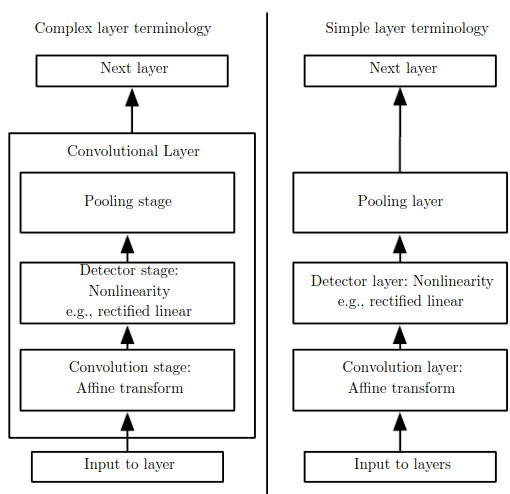
\includegraphics[width=0.6\textwidth,height=0.65\textheight,keepaspectratio]{images/marcoteorico/types}
		\end{center}
		
		\begin{center}
		\caption{\tiny{Terminología de capas complejas(izquierda) y de capas simples(derecha)}}
		\vskip -0.25cm
		{\tiny{Fuente: \citep{Goodfellow-et-al-2016}}}
		\end{center}
		%\vspace{-1.5em}
		\end{figure}
	\end{itemize}
}
%-----------------%----Arquitectura del Modelo-----%-----------------
\subsection{Arquitectura del Modelo}
\frame{
\begin{block}
{\Large{Arquitectura del Modelo}}
\end{block}
		\begin{itemize}
			\item<1->La arquitectura de la red está inspirada en el arquitectura Inception \citep{Inception} y en la arquitectura AlexNet\citep{Krizhevsky2012} para la clasificación de imágenes. En la arquitectura Inception, el modelo creado es denominado GoogLeNet, similar a AlexNet donde varios módulos iniciales son apilados uno sobre el otro para producir el resultado final. En el módulo de inicio, en ese tipo de red se usaron diversos tamaños de filtros convolucionales para capturar características de diferente abstracción. 
			\vskip 0.5cm
			\item<2-> El alto nivel de abstracción se captura con filtros de mayor tamaño y el de un nivel inferior con filtros de menor tamaño. Procesando información visual a diferentes escalas y al concatenarlas se obtiene un nivel eficiente de abstracción. 
		\end{itemize}
}



\frame{
\begin{block}
{\Large{Arquitectura del Modelo}}
\end{block}
		\begin{itemize}
		\vskip 0.5cm
		\item<1-> En esta investigación se utilizó una versión modificada de las arquitecturas antes mencionadas. Se incorporó {\bf funciones de escala-múltiple} \citep{Multi_scale_feat}, lo que significa que la salida de las capas convolucionales no solo se envía a la capa posterior, sino que también se ramifica y se introduce al clasificador (capa totalmente conectada). La razón detrás de esto es que cuando el clasificador está tomando una decisión basada en convoluciones, podría encontrar que la salida de la primera o segunda capa convolucional también es útil. Básicamente con las características de escala múltiple depende del clasificador qué nivel de abstracción usar, ya que tiene acceso a las salidas de todas las capas convolucionales, es decir, características en todos los niveles de abstracción.

		% Estas capas ramificadas se someten a un pooling máximo adicional, de modo que todas las convoluciones se submuestrean proporcionalmente antes de entrar en el clasificador. Así se garantiza que todas las funciones de escala múltiple experimenten la misma cantidad de máximo aprovechamiento.

		\end{itemize}
}


\frame{
\begin{block}
{\Large{Arquitectura del Modelo}}
\end{block}
		\begin{figure}[H]
		%\begin{center}
		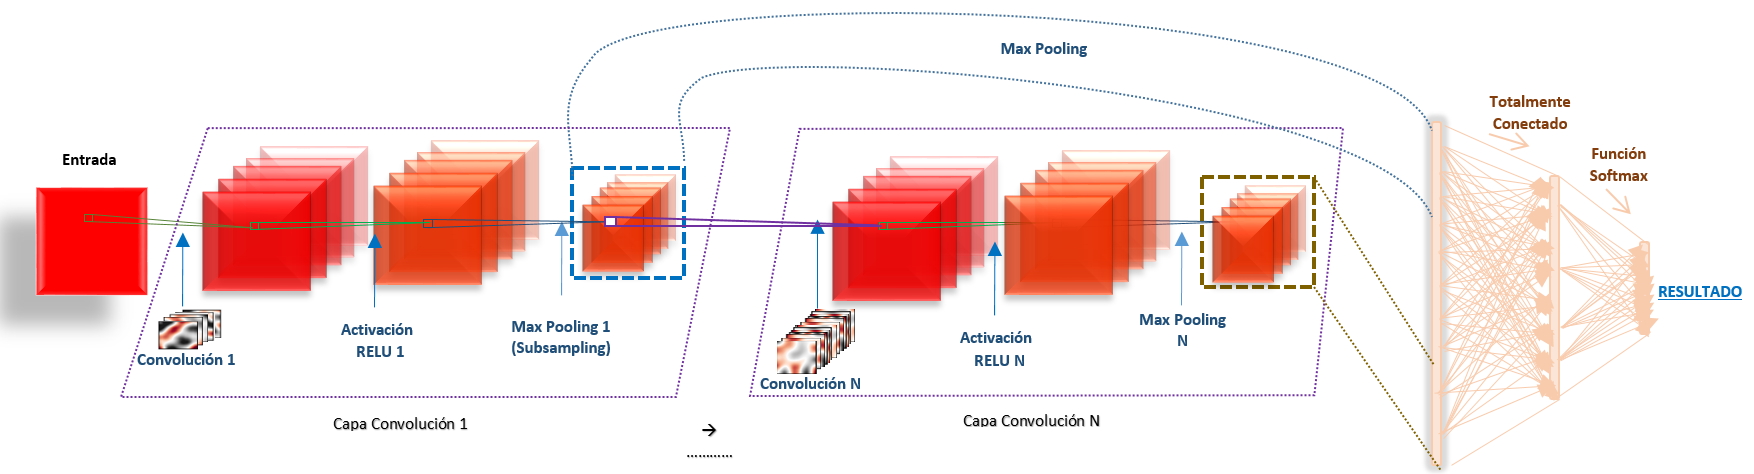
\includegraphics[width=1\textwidth]{images/desarrollo/networkArquitec/designNet}
		%\end{center}
		\begin{center}
		\caption{\small{Modelo del diseño de la Red propuesta}}
		
		{\small{\fontsize{10}{16.8}\selectfont {Fuente propia}}}
		\end{center}
		\vspace{-1.5em}
		\end{figure}
}


%-----------------%----Componentes del Modelo-----%-----------------
\subsection{Componentes del Modelo}
\frame{
\begin{block}
{\Large{Componentes del Modelo}}
\end{block}
		\begin{itemize}
			\item<1->Capa Convolucional
			\vskip 0.5cm
			\item<2-> Capa de Activación ReLU(Rectified Linear Units)
			\vskip 0.5cm
			\item<3-> Capa de Agrupación(Pooling)
			\vskip 0.5cm
			\item<4-> Capa totalmente conectada (Fully-connected layer)
		\end{itemize}
}
%--------------------------------------Capa Convolucional------------------------------
%\subsubsection{Capa Convolucional}
\frame{
\begin{block}
{\Large{Capa Convolucional}}
\end{block}
		\begin{itemize}
			\item<1->Los parámetros de la capa convolucional consisten basicamente en dos datos. La entrada y todo lo que respecta a un conjunto de filtros(también denomidados kernels) cuyos valores se aprenden, es decir, empiezan con datos aleatorios y conforme avance el entrenamiento se van alterando. 
			\vskip 0.5cm
			\item<2-> Durante el proceso hacia adelante, se desliza (más precisamente, convolve) cada filtro a través del ancho y alto del volumen de entrada para calcular los productos de puntos entre las entradas del filtro y la entrada en cualquier posición.
		\end{itemize}
}

\frame{
\begin{block}
{\Large{Capa Convolucional}}
\end{block}

		\begin{figure}[H]
			\begin{center}
			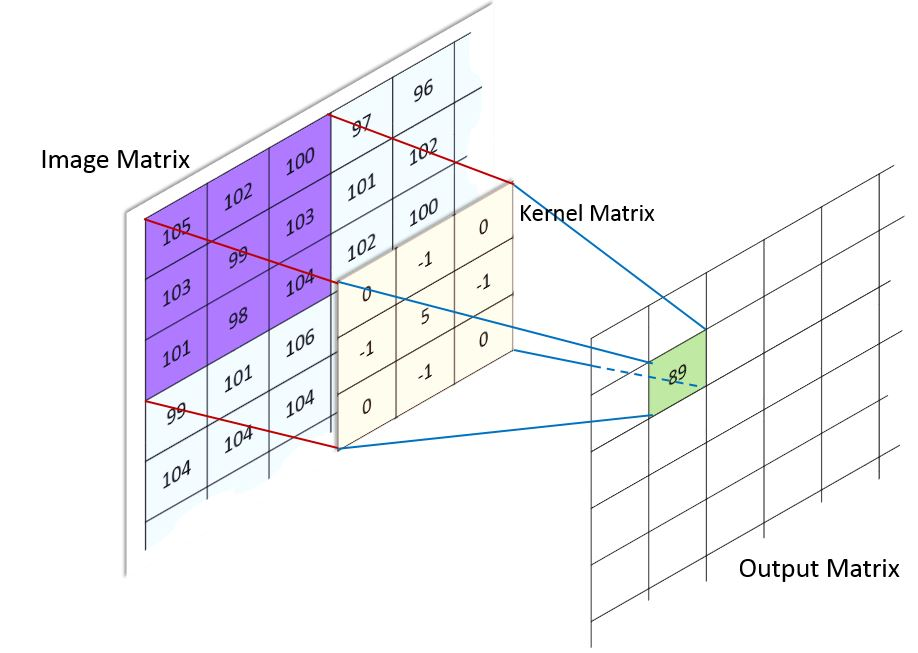
\includegraphics[width=0.75\textwidth,height=0.5\textheight,keepaspectratio]{images/marcoteorico/Convolution_calculation1}
			\end{center}
			\begin{center}
			\caption{\tiny{Posicionamiento del kernel/filtro por pixel}}
			{\tiny{Fuente: Fuente Propia}}
			\end{center}
			
		\end{figure}
}


\frame{
\begin{block}
{\Large{Capa Convolucional}}
\end{block}

		\begin{itemize}
			\item<1->A medida que deslizamos el filtro sobre el ancho y la altura del volumen de entrada produciremos un mapa de activación bidimensional que proporciona las respuestas de ese filtro en cada posición espacial. Por lo que simplemente se multiplica cada píxel en el filtro por el valor del píxel en la imagen. Para luego, sumar las respuestas y dividirlas por el número total de píxeles en el filtro. 
		
		%\item<3->
		\begin{figure}[H]
		\begin{center}
		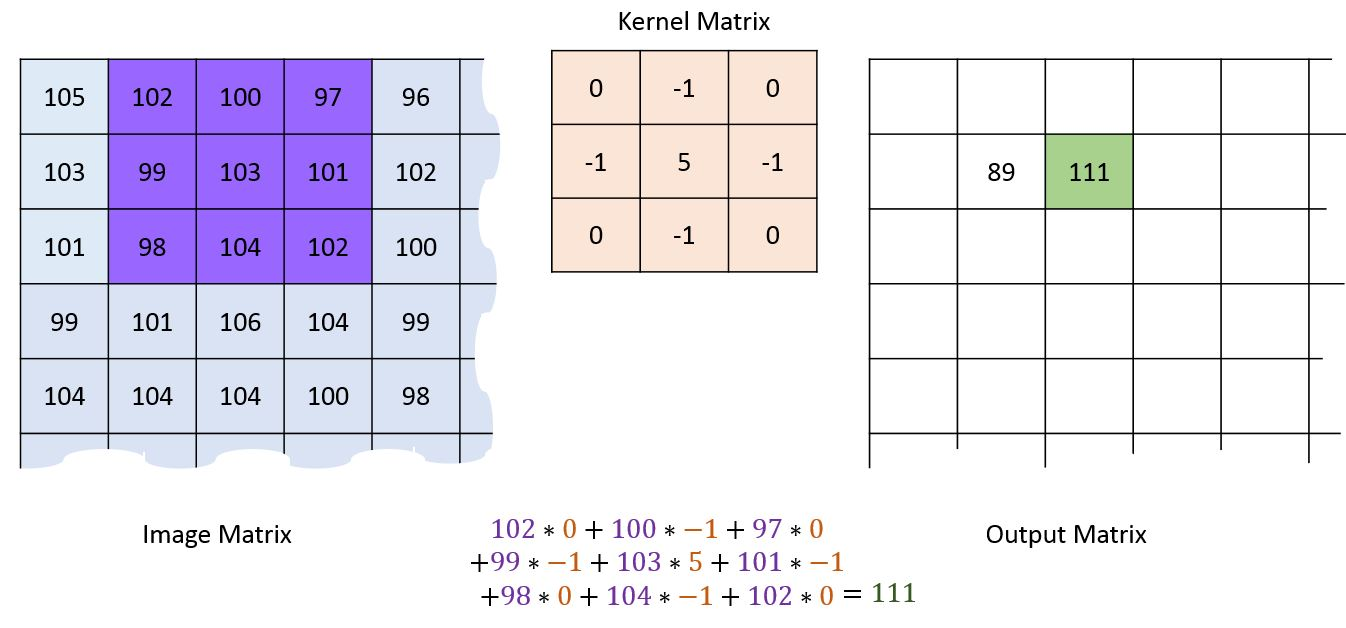
\includegraphics[width=0.75\textwidth,height=0.4\textheight,keepaspectratio]{images/marcoteorico/Convolution_calculation2}
		\end{center}
		\begin{center}
		\caption{\tiny{Cálculo Convolucional}}
		{\tiny{Fuente: Fuente Propia}}
		\end{center}
		
		\end{figure}

		\end{itemize}
}


\frame{
\begin{block}
{\Large{Capa Convolucional}}
\end{block}

		\begin{itemize}
			\item<2->Intuitivamente, la red aprenderá los filtros que se activan cuando ven algún tipo de característica visual, como un borde o contorno en alguna orientación específica. Debido a que la convolución aprovecha tres ideas importantes que pueden ayudar a mejorar un sistema de aprendizaje automático: 
			\begin{itemize}
			\item<3-> Interacciones dispersas
			\item<4-> Uso compartido de parámetros
			\item<5-> Representaciones equivalentes
			\end{itemize}
		\end{itemize}

}

\frame{
\begin{block}
{\Large{Capa Convolucional}}
\end{block}
		\begin{itemize}
	\item<1-> {\bf Capa Convolucional - Interacciones dispersas}
	%\vskip 0.5cm
			\begin{figure}[H]
		\begin{center}
		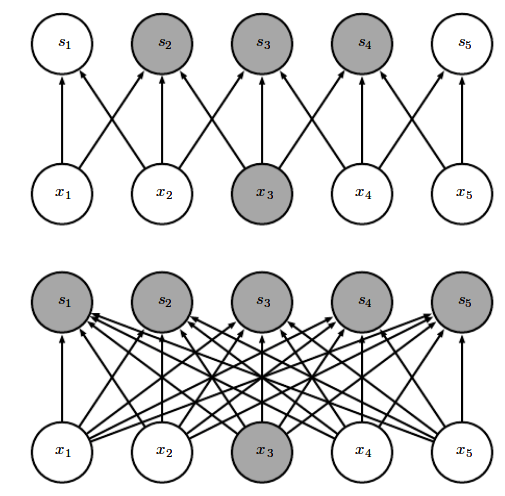
\includegraphics[width=0.5\textwidth,height=0.4\textheight,keepaspectratio]{images/marcoteorico/sparceCon}
		\end{center}
		
		\begin{center}
		\caption{\footnotesize \small{Conectividad dispersa vs No dispersa}}
		\vskip -0.3cm  
		{\small{Fuente:\citep{Rohrer}}}
		\end{center}
		\end{figure} 
		 Cuando {\bf {\textit {s}}} está formado por convolución con un kernel de ancho 3, solo tres salidas se ven afectadas por {\bf \textit  x}. (Abajo) Cuando {\bf \textit s} está formado por la multiplicación de la matriz, la conectividad ya no es dispersa, por lo que todos los resultados se ven afectados por $x_{3}$.
	\end{itemize}
}

\frame{
\begin{block}
{\Large{Capa Convolucional}}
\end{block}
		\begin{itemize}
	\item<1-> {\bf Capa Convolucional - Interacciones dispersas}
	 	\begin{itemize}
	 		\vskip 0.5cm
	 	\item<2->Esto significa que necesitamos almacenar menos parámetros, lo que reduce los requisitos de memoria del modelo y mejora su eficiencia estadística. También significa que el cálculo de la salida requiere menos operaciones, \citep{Goodfellow-et-al-2016}.
		\end{itemize}
	\end{itemize}
}

\frame{
\begin{block}
{\Large{Capa Convolucional}}
\end{block}
		\begin{itemize}
	\item<1-> {\bf Capa Convolucional - Uso compartido de parámetros}
	 	\begin{itemize}
	 		\vskip 0.5cm
	 	\item<2->En una red neuronal convolucional, cada miembro del kernel se utiliza en cada posición de la entrada (excepto tal vez algunos de los píxeles de los bordes, dependiendo de las decisiones de diseño con respecto al límite). El uso compartido de parámetros utilizado por la operación de convolución significa que en lugar de aprender conjuntos de parámetros para cada ubicación por separado, aprendemos un solo conjunto por kernel, \citep{Goodfellow-et-al-2016}.
		\end{itemize}
	\end{itemize}
}

\frame{
\begin{block}
{\Large{Capa Convolucional}}
\end{block}
		\begin{itemize}
	\item<1-> {\bf Capa Convolucional - Representaciones equivalentes}
	 	\begin{itemize}
	 		\vskip 0.5cm
	 	\item<2->La forma particular de compartir los parámetros hace que la capa tenga una propiedad llamada {\bf representaciones equivalentes}. Decir que una función es equivalente significa que si la entrada cambia, la salida cambia de la misma manera.
	 	\vskip 0.3cm
	 	\item<3->La convolución crea un mapa en 2-D de donde aparecen ciertas características en la entrada. Si movemos el objeto en la entrada, su representación se moverá la misma cantidad en la salida.
		\end{itemize}
	\end{itemize}
}

%Por ejemplo, al procesar imágenes, es útil detectar bordes en la primera capa de una red convolucional. Los mismos bordes aparecen más o menos en todas partes en la imagen, por lo que es práctico compartir los parámetros en toda la imagen.


\frame{
\begin{block}
{\Large{Capa Convolucional}}
\end{block}
	\begin{itemize}
	\item<1-> {\bf Capa Convolucional - Representaciones equivalentes}
	 	\begin{figure}[H]
		\begin{center}
		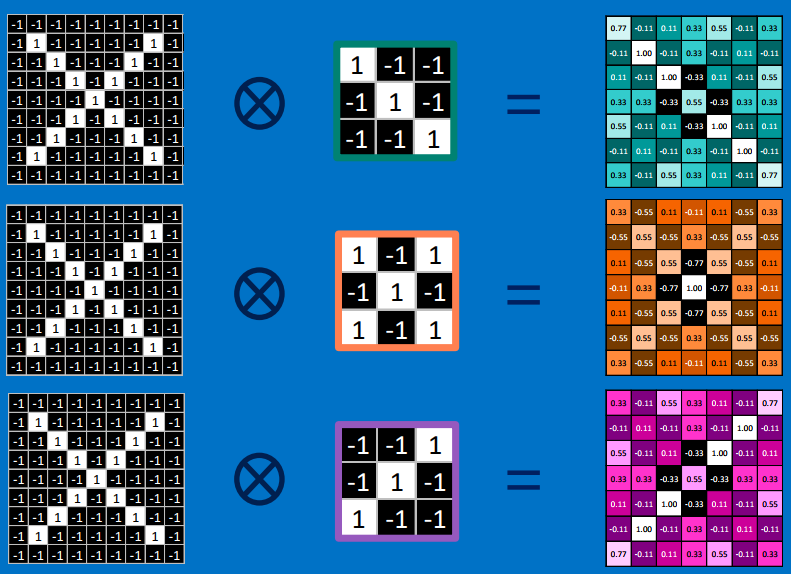
\includegraphics[width=0.6\textwidth,height=0.4\textheight,keepaspectratio]{images/marcoteorico/result_conv}
		\end{center}
		\begin{center}
		\vskip 0.1cm  
		\caption{\small{Resultado de Convolución(conjunto de mapas de activación. generado a partir de 3 filtros para 3 carecteristicas: diagonal derecha, cruzamiento central y diagonal izquierda). Simbolo de convolución: $\otimes$}}
		\vskip -0.1cm  
		{\small{Fuente: \citep{Rohrer}}}
		\end{center}
		\end{figure}

	\end{itemize}
}

%-----------------------------------------------------------------------------------

\frame{
\begin{block}
{\Large{Capa Convolucional}}
\end{block}
	\begin{itemize}
	\item<1-> {\bf Capa Convolucional - Construcción de un filtro o kernel}
		\setbeamertemplate{enumerate items}[square]
		\setbeamercolor{item projected}{bg=green!70!black,fg=blue}
	 	\begin{enumerate}
			\item La extensión espacial es el tamaño del filtro, comúnmente es de tamaño impar tanto en largo y ancho.
			
			\item El stride es otra pieza del bloque de construcción básico de los filtros convolucionales. Este representa el {\textit 'paso'} en la operación de convolución indicando cuánto es que se debe desplazar un filtro en una imagen con cada paso. El filtro se desliza sobre la imagen, se detiene en cada longitud de salto y realiza las operaciones necesarias en ese paso.

				\begin{figure}[H]
				\begin{center}
				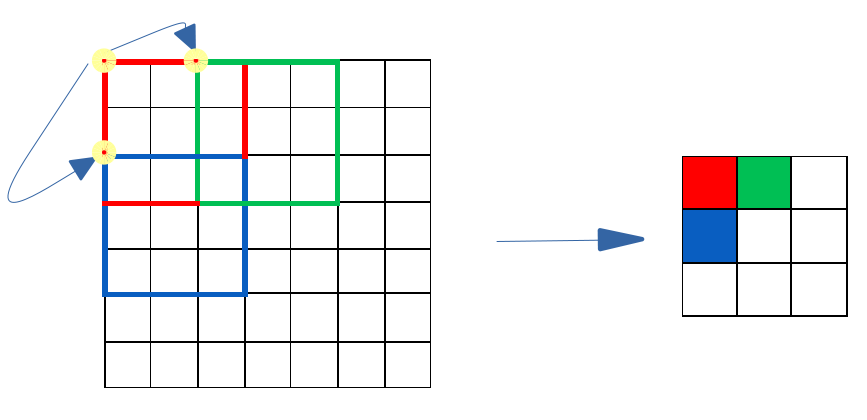
\includegraphics[width=0.65\textwidth,height=0.3\textheight,keepaspectratio]{images/marcoteorico/stride}
				\end{center}
				\begin{center}
				\caption{\tiny{Imagen con stride igual a 2, para el filtro tanto en largura como anchura}}
				\vspace{-0.5em}
				{\tiny{Fuente propia}}
				\end{center}
				\end{figure}
			\end{enumerate}
	\end{itemize}
}

\frame{
\begin{block}
{\Large{Capa Convolucional}}
\end{block}
	\begin{itemize}
	\item<1-> {\bf Capa Convolucional - Construcción de un filtro o kernel}
	 	\setbeamertemplate{enumerate items}[square]
	 	\setbeamercolor{item projected}{bg=green!70!black,fg=blue}
	 	\begin{enumerate}\addtocounter{enumi}{2}
			\item Zero-padding agrega ceros alrededor del borde de una imagen.
				\begin{figure}[H]
				\begin{center}
				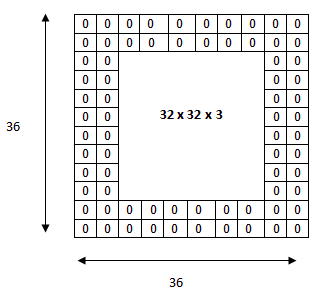
\includegraphics[width=0.4\textwidth]{images/marcoteorico/PAD2}
				\end{center}
				\begin{center}
				\caption{\tiny{Ejemplo de zero-padding con tamaño 2}}
				\vspace{-0.5em}
				{\tiny{Fuente propia}}
				\end{center}
				\end{figure}
		\end{enumerate}
	\end{itemize}
}

%Los principales beneficios del relleno son los siguientes:
%\item Le permite usar una capa de convolución sin necesariamente reducir la altura y el ancho de los volúmenes. Esto es importante para construir redes más profundas, ya que de lo contrario la altura / ancho se reduciría a medida que se avanza hacia capas más profundas.
%\item Nos ayuda a mantener más información en el borde de una imagen. Sin relleno, muy pocos valores en la siguiente capa se verían afectados por los píxeles como los bordes de una imagen.

\frame{
\begin{block}
{\Large{Capa Convolucional}}
\end{block}
		\begin{itemize}
		\item<1-> {\bf Capa Convolucional - Ecuación de Convolución}
	

	 	\vskip 0.5cm
	 	\item<2->	
		\begin{center}
		${conv_j^n} ={\sum_{k=1}^k x_k^n \times w_{kj} ^n + b_n}$
		\end{center}
		
		En el que:\vskip 0.1cm
		\begin{itemize}
			\item $x$ son valores de entrada
			\item $w,b$ pesos y biases(sesgos) del kernel, respectivamente
			\item $n$ es el número de la capa
			\item $j$ es el número del filtro de salida
			\item $k$ es la cantidad de filtros en la capa $n-1$ o $n$
		\end{itemize}

		
	\end{itemize}
}

\frame{
\begin{block}
{\Large{Capa Convolucional}}
\end{block}
	

		\begin{figure}[H]
		\begin{center}
		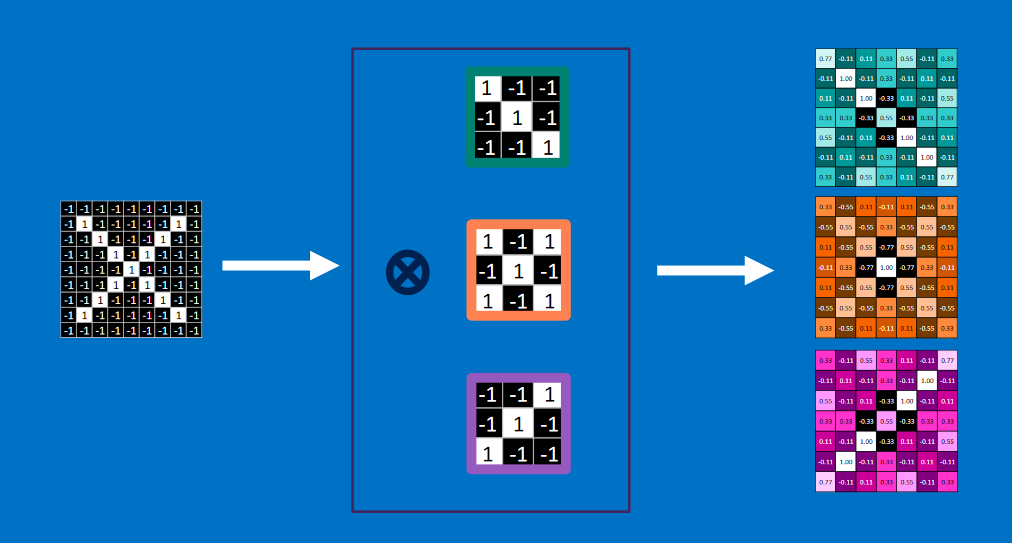
\includegraphics[width=0.8\textwidth]{images/marcoteorico/endofConv}
		\end{center}
		\begin{center}
		\caption{\tiny{Resultado Final de Convolución}}
		\vspace{-0.5em}
		{\tiny{Fuente: \citep{Rohrer}}}
		\end{center}
		\end{figure}

}

%----------------------------------------------Capa ReLU(Rectified Linear Units)------------

\frame{
\begin{block}
{\Large{Capa ReLU(Rectified Linear Units)}}
\end{block}
		\begin{itemize}
			\item<1->Una red neuronal artificial consiste básicamente en multiplicaciones y suma de matrices. Si solo utilizáramos estos cálculos lineales, podríamos apilarlos uno encima del otro y esa no sería una red muy profunda. Por lo tanto, a menudo se utiliza funciones de activación no lineales en cada capa de la red.
			\vskip 0.3cm
			\item<2-> Estas son las tres funciones de activación no lineal más populares:
				\begin{enumerate}
				\item[1)] Sigmoid (analiza un valor entre 0 y 1)  
				\item[2)] TanH (analiza un valor entre -1 y 1) 
				\item[3)] ReLU (si el valor es negativo, se convierte en 0, de lo contrario, permanece igual) 
				\end{enumerate}

				\begin{figure}[H]
%				\begin{center}
				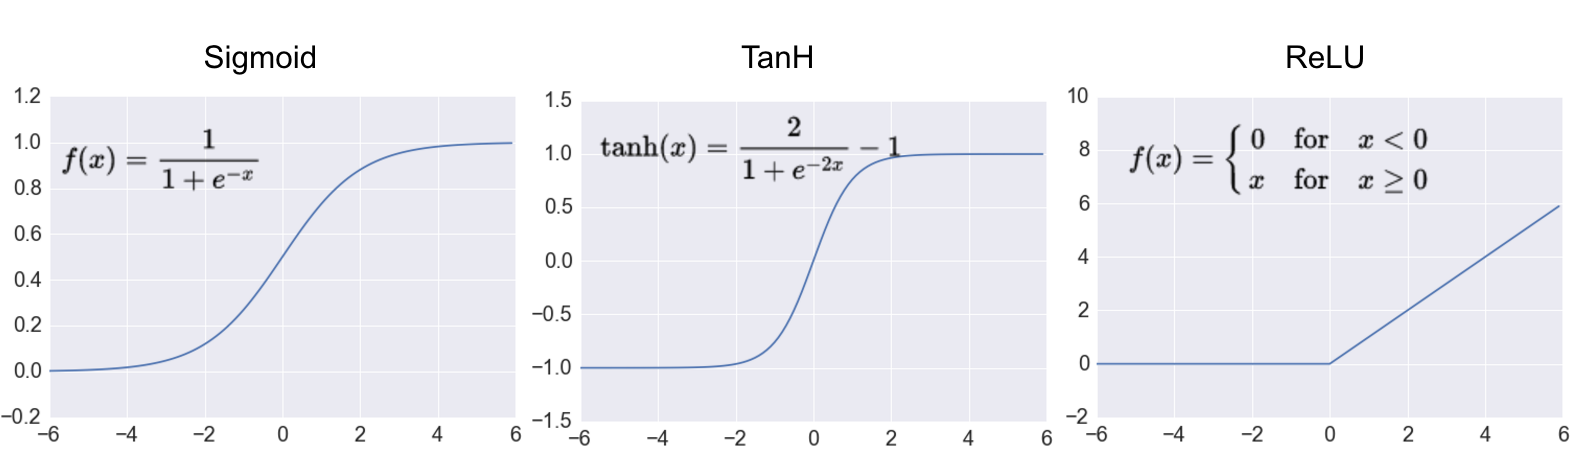
\includegraphics[width=0.8\textwidth,height=0.3\textheight,keepaspectratio]{images/marcoteorico/activfunct}
%				\end{center}
				%\begin{center}
				%\caption{\tiny{Funciones de activación}}
				%\vskip -0.2cm  
				%{\tiny{Fuente propia}}
				%\end{center}
				
				\end{figure}

		\end{itemize}
}


\frame{
\begin{block}
{\Large{Capa ReLU(Rectified Linear Units)}}
\end{block}
		
 	\begin{itemize}
 		%\vskip 0.5cm
 	\item<1->Actualmente, ReLU es la función de activación no lineal más utilizada \citep{cs231n}, que básicamente aplica la función ${f(x)} = {max (0, x)} $ a todos los valores en el volumen de entrada.
		\begin{itemize}
			\item<2->La red puede entrenar mucho más rápido (debido a la eficiencia computacional) sin hacer una diferencia significativa en la precisión.
			\vskip 0.3cm
			\item<3->Alivia el problema del gradiente de fuga, que es el problema donde las capas inferiores de la red entrenan muy lentamente porque el gradiente de optimización	disminuye exponencialmente a través de las capas.
		\end{itemize}
	\item<4->El hecho de que entradas en la función de activación de valores menores o iguales a cero resulten cero, induce a la dispersión en las unidades ocultas, que según lo comentado anteriormente, produce representaciones dispersas las cuales se consideran más valiosas, \citep{RELU}. 
	\end{itemize}
}

\frame{
\begin{block}
{\Large{Capa ReLU(Rectified Linear Units)}}
\end{block}
				\begin{figure}[H]
		\begin{center}
		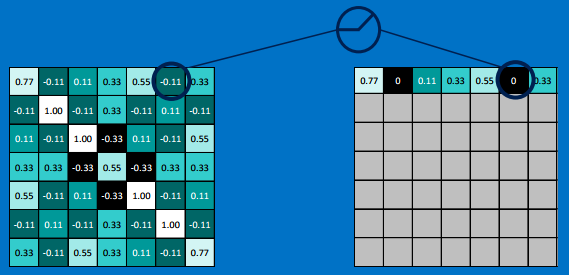
\includegraphics[width=0.6\textwidth,height=0.5\textheight,keepaspectratio]{images/marcoteorico/relu}
		\end{center}
		\begin{center}
		\caption{\small{Procedimiento de la función ReLU}}
		\vskip -0.2cm  
		{\small{Fuente: \citep{Rohrer}}}
		\end{center}
		\vspace{-1.5em}
		\end{figure}
}

\frame{
\begin{block}
{\Large{Capa ReLU(Rectified Linear Units)}}
\end{block}
				\begin{figure}[H]
		\begin{center}
		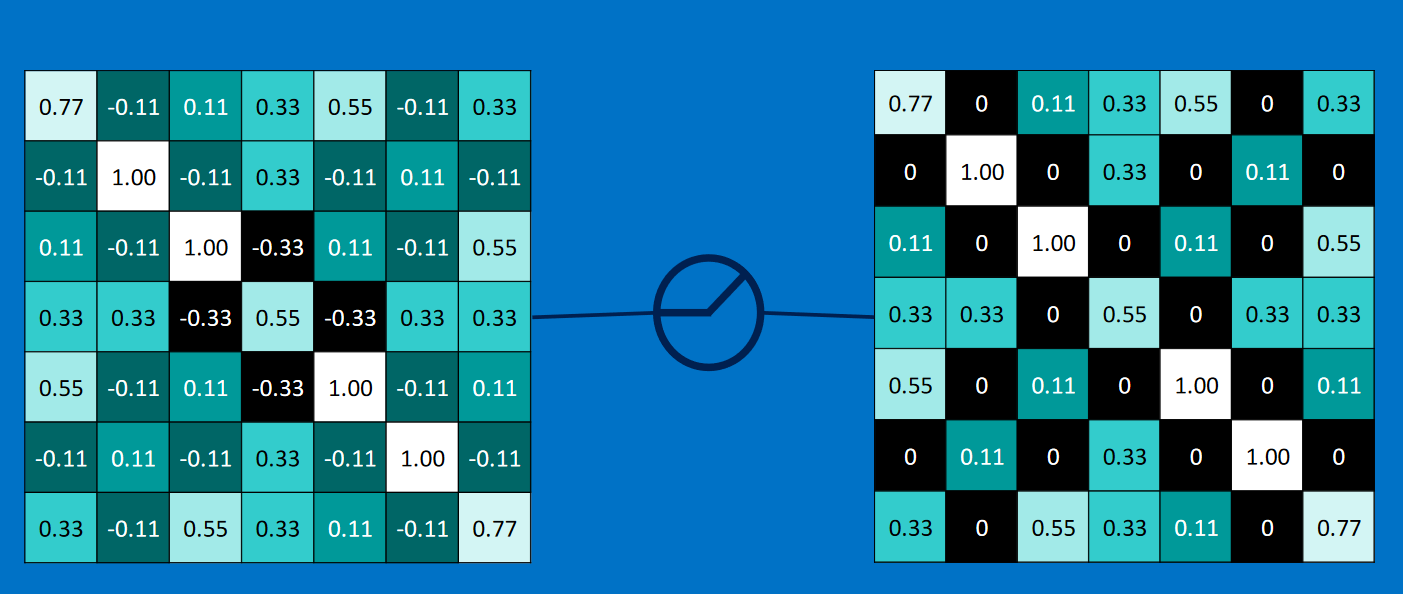
\includegraphics[width=0.6\textwidth,height=0.6\textheight,keepaspectratio]{images/marcoteorico/relu2}
		\end{center}
		\begin{center}
		\caption{\small{Procedimiento de la función ReLU}}
		\vskip -0.2cm  
		{\small{Fuente: \citep{Rohrer}}}
		\end{center}
		\vspace{-1.5em}
		\end{figure}
}

\frame{
\begin{block}
{\Large{Capa ReLU(Rectified Linear Units)}}
\end{block}
				\begin{figure}[H]
		\begin{center}
		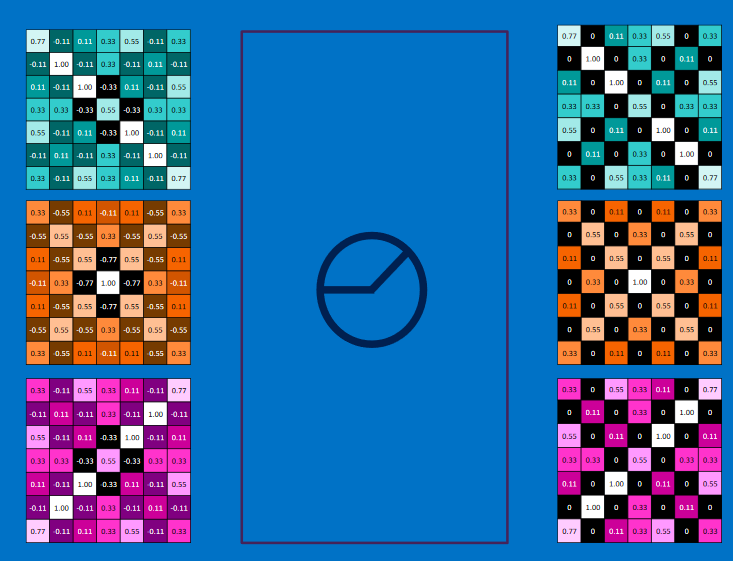
\includegraphics[width=0.6\textwidth,height=0.5\textheight,keepaspectratio]{images/marcoteorico/relu3}
		\end{center}
		\begin{center}
		\caption{\small{Procedimiento de la función ReLU}}
		\vskip -0.2cm  
		{\small{Fuente: \citep{Rohrer}}}
		\end{center}
		\vspace{-1.5em}
		\end{figure}
}
%---------------------------------------------Técnica Dropout------------
\frame{
\begin{block}
{\Large{Técnica Dropout}}
\end{block}
		
 	\begin{itemize}
 		%\vskip 0.5cm
 	\item<1-> Es una técnica de regularización que tiene por objetivo de reducir el sobreajuste que puede darse durante el entrenamiento de una red neuronal. Consiste en establecer a cero la salida de cada neurona oculta con una probabilidad 0.5(comúnmente). Las neuronas que se abandonan de esta manera no contribuyen al pase directo y no participan en las siguientes etapas de entrenamiento.
		\begin{figure}[H]
		\begin{center}
		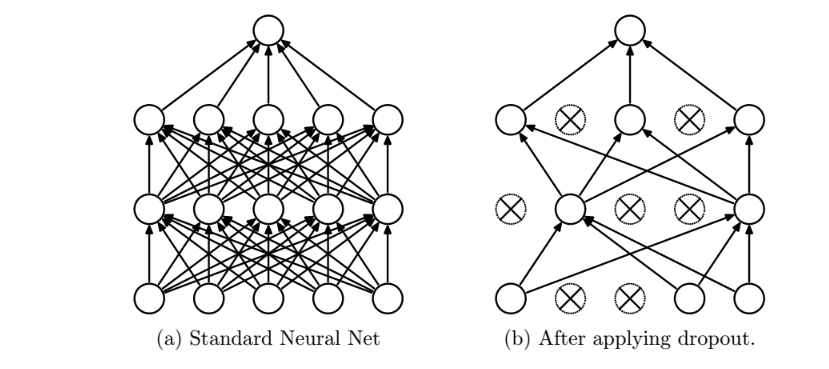
\includegraphics[width=0.6\textwidth,height=0.5\textheight,keepaspectratio]{images/marcoteorico/dropout_sample}
		\end{center}
		\begin{center}
		\caption{\tiny{En la izquierda la red neuronal común y a la derecha la red neuronal diluida producida por la aplicación de dropout}}
		{\tiny{\citep{AulaDNN}}}
		\end{center}
		\end{figure}
	\end{itemize}
}

\frame{
\begin{block}
{\Large{Técnica Dropout}}
\end{block}
		
 	\begin{itemize}
 		%\vskip 0.5cm
 	\item<1->Por lo tanto, cada vez que se presenta una entrada, la red neuronal muestra una arquitectura diferente, pero todas estas arquitecturas comparten ponderaciones. Esta técnica reduce las coadaptaciones complejas de las neuronas, ya que una neurona no puede depender de la presencia de otras neuronas particulares. Por lo tanto, se ve forzado a aprender características más robustas que son útiles en conjunción con muchos subconjuntos aleatorios diferentes de las otras neuronas.
	\begin{figure}[H]
		\begin{center}
		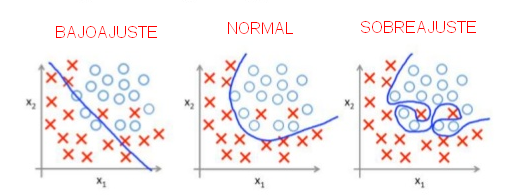
\includegraphics[width=0.6\textwidth,height=0.5\textheight,keepaspectratio]{images/marcoteorico/dropout}
		\end{center}
		\begin{center}
		\caption{\tiny{Procesos que pueden ocurrir durante entrenamiento. Dropout evita el sobreajuste}}
		\vskip -0.3cm  
		{\tiny{Fuente propia}}
		\end{center}
		
		\end{figure}
	\end{itemize}
}

%----------------------------------Capa de Agrupación(Pooling)-------------------------		

\frame{
\begin{block}
{\Large{Capa de Agrupación(Pooling)}}
\end{block}
		
 	\begin{itemize}
 		%\vskip 0.5cm
 	\item<1->Una variedad de cálculos que reducen la dimensionalidad de un mapa de características se conocen como agrupación. La agrupación, que se aplica a cada canal por separado, permitiendo que la red sea robusta e invariante a pequeños cambios y distorsiones.
 	\vskip 0.2cm  
 	\item<2->La capa Pooling(también conocida como una capa de reducción de resolución) combina o agrupa, un conjunto de valores en su campo receptivo en un menor número de valores.
	\vskip 0.2cm  
 	\item<3->Puede ser configurado en función del tamaño de su campo receptivo (por ejemplo, 2 x 2) y en función a la operación de agrupamiento (por ejemplo, máximo-max o promedio-average).
		\begin{figure}[H]
		\begin{center}
		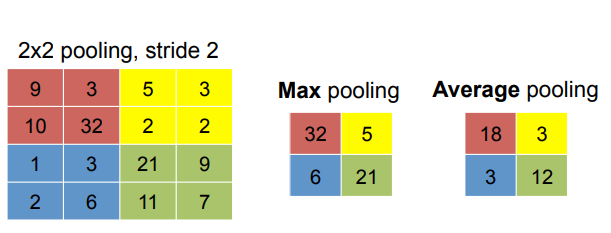
\includegraphics[width=0.4\textwidth,height=0.4\textheight,keepaspectratio]{images/marcoteorico/pooling}
		\end{center}
		\begin{center}
		\caption{\tiny{Formas de agrupamiento(pooling)}}
		\vskip -0.2cm  
		{\tiny{Fuente: \citep{caffe}}}
		\end{center}
		\end{figure}
	\end{itemize}
}

% esto se ejecuta con dos objetivos, el primero de reducir la cantidad de parámetros y el cálculo en la red. El segundo es que controlará el sobreajuste.

\frame{
\begin{block}
{\Large{Capa de Agrupación(Pooling)}}
\end{block}
		
 	\begin{itemize}
 		%\vskip 0.5cm
 	\item<1-> El  Max-pooling  es la más popular reduciendo progresivamente el tamaño espacial de la representación de una imágen(mapa de características) mientras conserva la información más importante en ella. El proceso matematico consiste en pasar una pequeña ventana(kernel) através de una imagen y tomar el valor máximo de la ventana en cada paso. 
 	\vskip 0.2cm  

		\begin{figure}[H]
		\begin{center}
		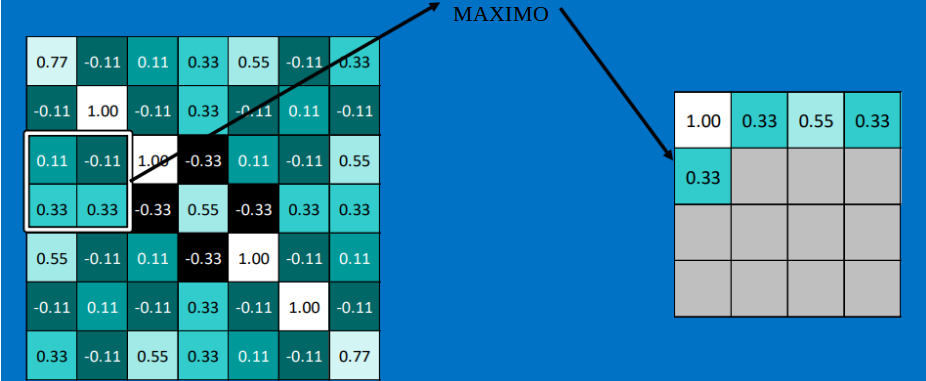
\includegraphics[width=0.5\textwidth,height=0.5\textheight,keepaspectratio]{images/marcoteorico/pool1}
		\end{center}
		\begin{center}
		\caption{\tiny{Operación MAX-pooling en capa de Agrupación}}
		\vskip -0.2cm  
		{\tiny{Fuente: \citep{Rohrer}}}
		\end{center}
		\end{figure}
	\end{itemize}
}

\frame{
\begin{block}
{\Large{Capa de Agrupación(Pooling)}}
\end{block}
		
 	\begin{itemize}
 		%\vskip 0.5cm
 	\item<1-> 
		Este proceso es aplicado para cada mapa de activación(salida de la capa de convolución). Análogamente con la capa de convolución, el resultado en esta capa es un conjunto de imágenes que muestran un versión agrupada de las imágenes de entrada. 
 	\vskip 0.2cm  

		\begin{figure}[H]
		\begin{center}
		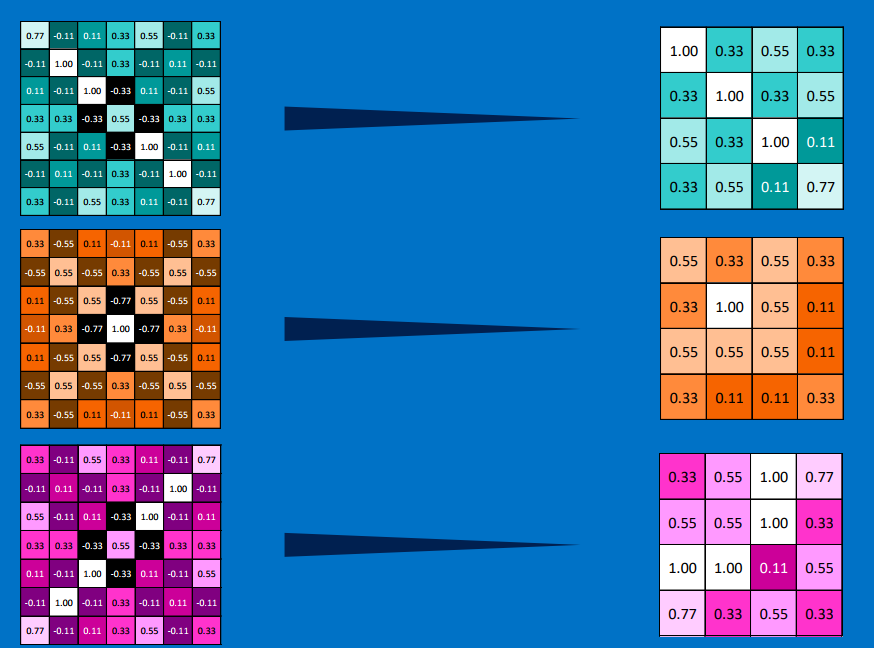
\includegraphics[width=0.6\textwidth,height=0.5\textheight,keepaspectratio]{images/marcoteorico/pool2}
		\end{center}
		\begin{center}
		\caption{\tiny{Resultado de Agrupación}}
		\vskip -0.2cm  
		{\tiny{Fuente: \citep{Rohrer}}}
		\end{center}
		\end{figure}
	\end{itemize}
}




\frame{
\begin{block}
{\Large{Componentes del Modelo - Capas Conectadas}}
\end{block}
		
 	\begin{itemize}
 		%\vskip 0.5cm
 	\item<1-> 
		Finalmente la salida de cada capa se convierte en entrada para una posterior.
 	\vskip 0.2cm  

		\begin{figure}[H]
		\begin{center}
		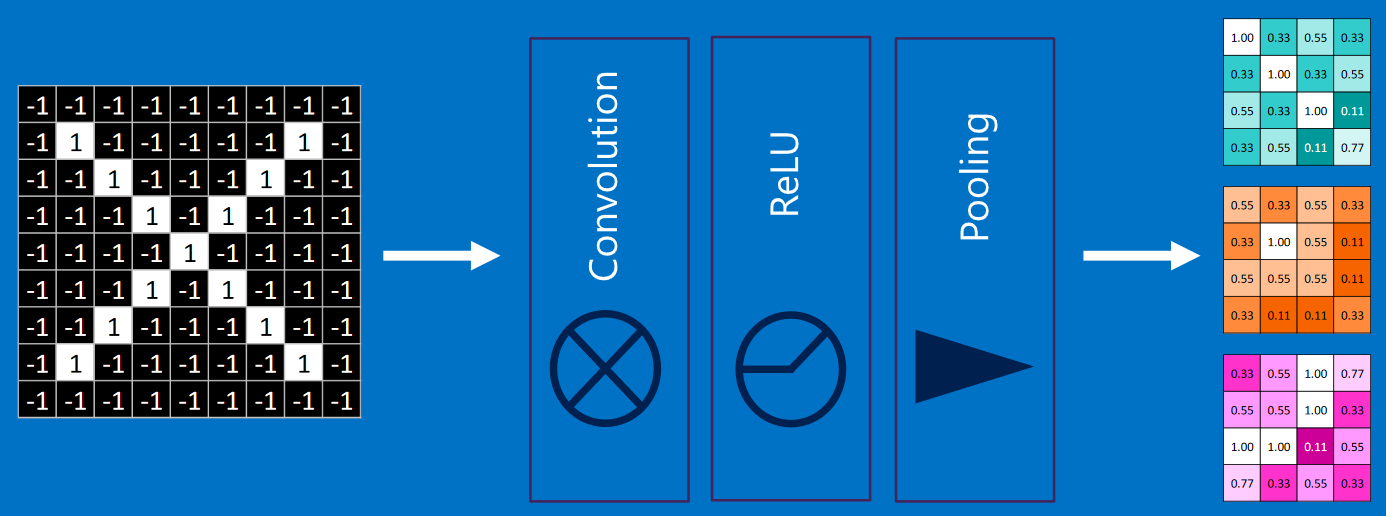
\includegraphics[width=0.9\textwidth,height=0.9\textheight,keepaspectratio]{images/marcoteorico/endofLayers1}
		\end{center}
		\begin{center}
		\caption{\tiny{Capas Apiladas}}
		\vskip -0.2cm  
		{\tiny{Fuente: \citep{Rohrer}}}
		\end{center}
		\end{figure}
	\end{itemize}
}


\frame{
\begin{block}
{\Large{Componentes del Modelo - Capas Conectadas}}
\end{block}
		
 	\begin{itemize}
 		%\vskip 0.5cm
 	\item<1-> 
		Las capas pueden ser repetidas múltiples veces.
 	\vskip 0.2cm  

		\begin{figure}[H]
		\begin{center}
		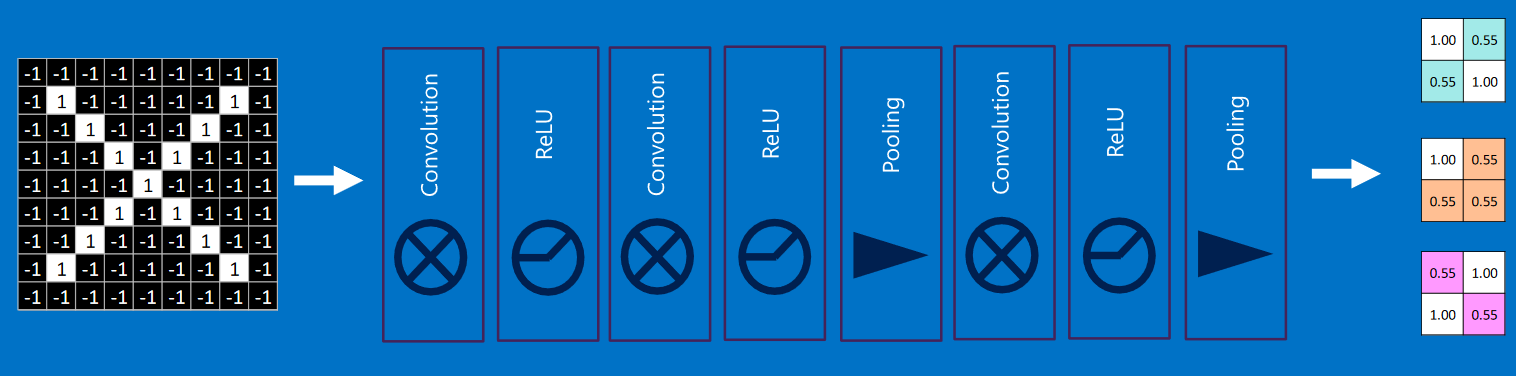
\includegraphics[width=0.8\textwidth,height=0.9\textheight,keepaspectratio]{images/marcoteorico/endofLayers2}
		\end{center}
		\begin{center}
		\caption{\tiny{Apilación Profunda de Capas}}
		\vskip -0.2cm  
		{\tiny{Fuente: \citep{Rohrer}}}
		\end{center}
		\end{figure}
	\end{itemize}
}








%---------------------Capa totalmente conectada )----------------------------------

\frame{
\begin{block}
{\Large{Capa totalmente conectada (Fully-connected layer)}}
\end{block}
		
 	\begin{itemize}
 		%\vskip 0.5cm
 	\item<1-> 
		Esta capa por lo general aparece al final de la arquitectura y es similar al Perceptrón multicapa(MultilayerPerceptron -MLP), en el cual la neurona de salida se conecta a todas las neuronas de entrada y el peso de las conexiones son actualizadas usando el método de retropropagación. 
 	\vskip 0.2cm  
		\begin{figure}[H]
		\begin{center}
		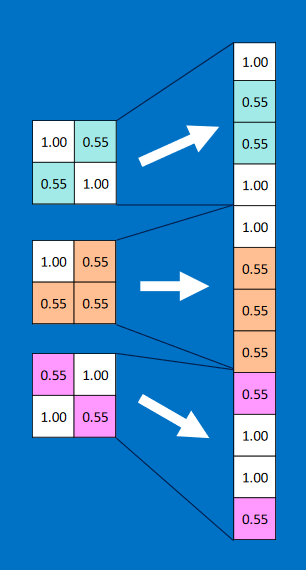
\includegraphics[width=0.4\textwidth,height=0.5\textheight,keepaspectratio]{images/marcoteorico/prevFC}
		\end{center}
		\begin{center}
		\caption{\tiny{Eventualmente, con un mapa de características lo suficientemente pequeño, el contenido se aplastará en un vector de una sola dimensión y será entrada para en un MLP totalmente conectado para su procesamiento}}
		\vskip -0.2cm  
		{\tiny{Fuente: \citep{Rohrer}}}
		\end{center}
		\end{figure}
	\end{itemize}
}


\frame{
\begin{block}
{\Large{Capa totalmente conectada (Fully-connected layer)}}
\end{block}
		
 	\begin{itemize}
 		%\vskip 0.5cm
 	\item<1-> En esta última capa del modelo generalmente se utiliza una función de activación diferente, porque en esta capa se pretende que tenga una salida determinada. La {\bf función softmax}, conocida tambien como función exponencial normalizada, es muy popular cuando se hace la clasificación.
 	\vskip 0.2cm  
 	\item<2->  La salida de una red neuronal completamente conectada no es una distribución de probabilidad, sin embargo, el uso de esta función ayuda a obternela. Por lo que esta función permitirá estimar la probabilidad de que la imagen de entrada pertenezca a cada una de las clases al realizar una normalización con el objetivo que el valor de cada neurona esté limitado entre cero y uno y así permitir que el resultado de las neuronas de salida sumen a uno, \citep{Bishop}. 
	\end{itemize}
}


%-------------------------------------------------------------------------------

\subsection{Validación Cruzada}
\frame{
\begin{block}
{\Large{Validación Cruzada}}
\end{block}
		
 	\begin{itemize}
 		%\vskip 0.5cm
 	\item<1-> La cantidad de errores en la votación, nos indica qué tan buenas son nuestras pesos y bias. Las características y los pesos se pueden ajustar para reducir el error. Cada valor se ajusta un poco más alto y un poco más bajo, y el nuevo error se calcula cada vez. 
 	\vskip 0.2cm  
 	\item<2->  Después de hacer esto para cada píxel de función en cada capa convolucional y cada peso en cada capa totalmente conectada, los nuevos pesos dan una respuesta que funciona ligeramente mejor para esa imagen, \citep{Bishop}. 
 	 	\vskip 0.2cm  
 	\item<3->   Esto se repite con cada imagen subsiguiente en el conjunto de imágenes etiquetadas. Los problemas que ocurren en una sola imagen se olvidan rápidamente, pero los patrones que aparecen en muchas imágenes se integran en las características y los pesos de conexión.
	\end{itemize}
}

\frame{
\begin{block}
{\Large{Validación Cruzada}}
\end{block}
		
 	\begin{itemize}
 		%\vskip 0.5cm
 	\item<1-> Para el entrenamiento, el conjunto de datos se divide en un subconjunto de entrenamiento y otro para validación. En esta investigación se dividirá el 75\% para entrenamiento y 75\% para validación.
 	\vskip 0.2cm  
 	\item<2->   La división en subgrupos de entrenamiento y validación generalmente se realiza de manera aleatoria, para garantizar que ambos subconjuntos sean muestras aleatorias de la misma distribución.
 
	\end{itemize}
}




\frame{
\begin{block}
{\Large{Validación Cruzada}}
\end{block}
		
 	\begin{itemize}
 		%\vskip 0.5cm
 	\item<1-> Para una red neuronal, normalmente verá la ecuación escrita en una forma donde $y$ es el vector de verdad y la variable $\hat{y}$ (o algún otro valor tomado directamente de la última salida de la capa) es la estimación, y se vería así para un solo ejemplo:
 	
			\begin{center}
			$L = - \mathbf{y} \cdot log({\hat{y}})$
			\end{center}
			%\begin{center}
			%{\small{El valor es independiente de cómo la probabilidad restante se divide entre clases incorrectas}}
			%\end{center}
	
 	\vskip 0.2cm  
 	\item<2->   A menudo esta ecuación es promediada sobre todos los ejemplos como una función de costo. No siempre se cumple estrictamente en las descripciones, pero generalmente una función de pérdida es de nivel inferior y describe cómo una sola instancia o componente determina un valor de error, mientras que una función de costo es de nivel superior y describe cómo se evalúa un sistema completo para la optimización. 
 	\vskip 0.2cm  
 	\item<3-> Una función de costo basada en pérdida de clasificación multiclase para un conjunto de datos de tamaño N podría verse así:
			\begin{center}
			$J = - \frac{1}{N}(\sum_{i=1}^{N} \mathbf{y_i} \cdot log({\hat{y}_i}))$
			\end{center}
		
	\end{itemize}
}

%----------------------------------------------------------------------------------

\frame{
\begin{block}
{\Large{Descenso de Gradiente}}
\end{block}
		
 	\begin{itemize}
 		%\vskip 0.5cm
 	\item<1-> Un gradiente mide cuánto cambia la salida de una función si se cambia un poco las entradas.

	\item<2->En el caso del entrenamiento de una red neuronal, el gradiente simplemente mide el cambio en todos los pesos con respecto al cambio en el error.
 	
	\item<3->El descenso de gradiente es un algoritmo de optimización iterativa utilizado al entrenar un modelo de aprendizaje automático, basado en una función convexa, que ajusta sus parámetros iterativamente para minimizar la función de pérdida(error) hasta su mínimo local.\citep{gradient}

	\item<4->La idea detrás del descenso de gradiente es disminuir de forma gradual, pero constante, el error de salida ajustando los pesos. Intuitivamente, se conoce que si un cambio en un peso aumentará (disminuirá) el error, entonces queremos disminuir (aumentar) ese peso. Matemáticamente, representa el cambio en el error dado un cambio de unidad en el peso:

		\begin{center}
		$ \frac{{\partial E}}{\partial w_{ij}}$
		\end{center}
		\begin{center}
		{\tiny{La derivada del error con respecto al peso}}
		\end{center}
	
	\end{itemize}
}
\frame{
\begin{block}
{\Large{Descenso de Gradiente}}
\end{block}
		
 	\begin{itemize}
 		%\vskip 0.5cm
 	\item<1-> Una vez que encontremos esta derivada, actualizamos el peso a través de lo siguiente:
 		\begin{center}
		$  \triangle w_{ij} = -\eta\frac{{\partial E}}{\partial w_{ij}} $
		\end{center}
		\begin{center}
		{\tiny{Representación de la distancia por la dirección del cambio. $\eta$  es tasa de aprendizaje}}
		\end{center}
		\vskip 0.2cm
	\item<2-> La tasa de Aprendizaje suele disminuir gradualmente durante las épocas de la fase de entrenamiento. Si actualizamos todos los pesos usando esta misma fórmula, esto equivale a moverse en la dirección de descenso más pronunciado a lo largo de la superficie de error, de ahí el nombre, descenso de gradiente.
	\end{itemize}
}
%----------------------------------------------------------------------------------

\frame{
\begin{block}
{\Large{Tasa de Aprendizaje (Learning Rate)}}
\end{block}
		
 	\begin{itemize}
 		%\vskip 0.5cm
 	\item<1-> Este parámetro puede entenderse como el tamaño del paso en la optimización para minimizar la función de pérdida de la red, es decir, es un parámetro que determina cuánto influye un paso de actualización en el valor actual de los pesos, por ejemplo, el tamaño del paso en el que el gradiente cae en la dirección máxima de la pendiente, \citep {AdamImg}.

		\begin{figure}[H]
		%\begin{center}
		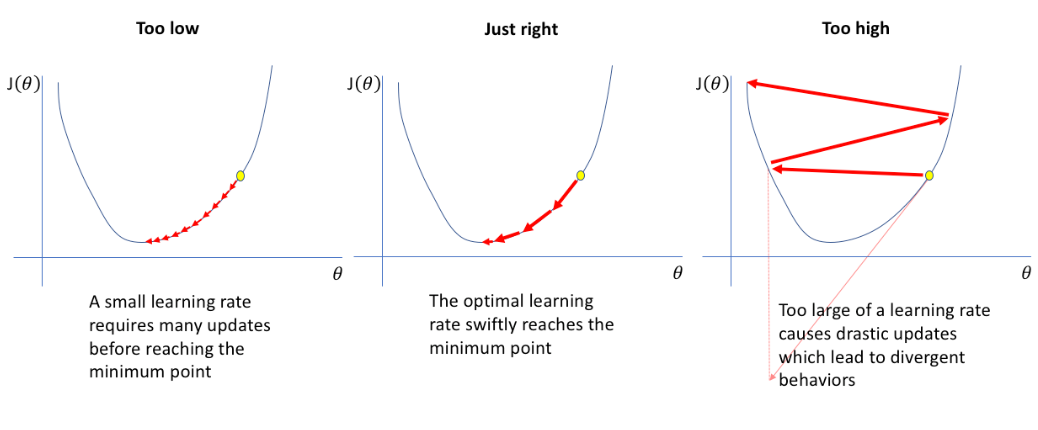
\includegraphics[width=1\textwidth]{images/desarrollo/entrenamiento/LR}
		%\end{center}
		\begin{center}
		\caption{\small{Establecimiento de la Tasa de Aprendizaje}}
		\vspace{-0.5em}
		{\small{\citep {AdamImg}}}
		\end{center}
		\end{figure}

 	%,height=0.5\textheight,keepaspectratio
			
	\end{itemize}
}
